\section{Partial\-Mapped\-Xover Class Reference}
\label{class_partial_mapped_xover}\index{PartialMappedXover@{PartialMappedXover}}
Partial Mapped Crossover.  


{\tt \#include $<$partial\_\-mapped\_\-xover.h$>$}

Inheritance diagram for Partial\-Mapped\-Xover::\begin{figure}[H]
\begin{center}
\leavevmode
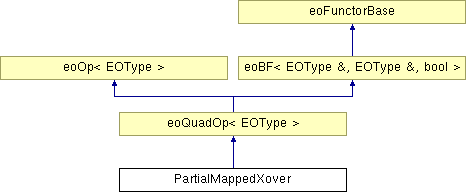
\includegraphics[height=4cm]{class_partial_mapped_xover}
\end{center}
\end{figure}
\subsection*{Public Member Functions}
\begin{CompactItemize}
\item 
bool \bf{operator()} (\bf{Route} \&\_\-\_\-route1, \bf{Route} \&\_\-\_\-route2)\label{class_partial_mapped_xover_1cda6ea86ca36e5de0125f4ba5cfc695}

\end{CompactItemize}
\subsection*{Private Member Functions}
\begin{CompactItemize}
\item 
void \bf{repair} (\bf{Route} \&\_\-\_\-route, unsigned \_\-\_\-cut1, unsigned \_\-\_\-cut2)\label{class_partial_mapped_xover_b6d4035544aff3b2b3fe4b0eeea185a2}

\end{CompactItemize}


\subsection{Detailed Description}
Partial Mapped Crossover. 



Definition at line 45 of file partial\_\-mapped\_\-xover.h.

The documentation for this class was generated from the following files:\begin{CompactItemize}
\item 
partial\_\-mapped\_\-xover.h\item 
partial\_\-mapped\_\-xover.cpp\end{CompactItemize}
